\documentclass[a4paper, 12pt]{article}
\usepackage{geometry}
\geometry{verbose,a4paper,tmargin=2cm,bmargin=2cm,lmargin=2cm,rmargin=2cm}
\usepackage[T2A]{fontenc}
\usepackage[utf8]{inputenc}
\usepackage[english,russian]{babel}
\newif\ifisinsp
\newif\ifisone
\newif\ifisname
\isinsptrue
\isonetrue
\isnamefalse
\def \labtype {Лабораторная}
% Это для нумерации страниц после титульника
\usepackage{fancyhdr}
\pagestyle{fancy}
\renewcommand{\headrulewidth}{0pt}
\fancyfoot[C] {\thepage}

\usepackage{hyperref}
\hypersetup{pdftex,colorlinks=true,allcolors=black}
\usepackage{hypcap}

\usepackage{graphicx}
\usepackage{adjustbox}
\usepackage{multirow}

\def \labtype {Курсовая}
\def \labsubj {Моделирование}
\def \labauthor {Айтуганов Д. А. \\ Чебыкин И. Б.}
\def \labgroup {P3301}
\def \labinsp {Муравьева-Витковская Л. А.}
\def \labname{Творческая работа: Моделирование многопроцессорного планировщика задач}
\isonefalse
\isnumfalse
\isnametrue

% https://en.wikibooks.org/wiki/LaTeX/Source_Code_Listings
\usepackage{listings}
\usepackage{color}
\definecolor{mygreen}{rgb}{0,0.6,0}
\definecolor{mygray}{rgb}{0.5,0.5,0.5}
\definecolor{mymauve}{rgb}{0.58,0,0.82}
\definecolor{lightgray}{rgb}{.9,.9,.9}
\definecolor{darkgray}{rgb}{.4,.4,.4}
\definecolor{purple}{rgb}{0.65, 0.12, 0.82}

\lstdefinelanguage{JavaScript}{
  keywords={typeof, new, true, false, catch, function, return, null, catch, switch, var, if, in, while, do, else, case, break},
  keywordstyle=\ttfamily\color{blue}\bfseries,
  ndkeywords={class, export, boolean, throw, implements, import, this},
  ndkeywordstyle=\ttfamily\color{darkgray}\bfseries,
  identifierstyle=\ttfamily\color{black},
  sensitive=false,
  comment=[l]{//},
  morecomment=[s]{/*}{*/},
  commentstyle=\color{purple}\ttfamily,
  stringstyle=\color{red}\ttfamily,
  morestring=[b]',
  morestring=[b]"
}


\lstdefinelanguage{CSS}{
  morekeywords={accelerator,azimuth,background,background-attachment,
    background-color,background-image,background-position,
    background-position-x,background-position-y,background-repeat,
    behavior,border,border-bottom,border-bottom-color,
    border-bottom-style,border-bottom-width,border-collapse,
    border-color,border-left,border-left-color,border-left-style,
    border-left-width,border-right,border-right-color,
    border-right-style,border-right-width,border-spacing,
    border-style,border-top,border-top-color,border-top-style,
    border-top-width,border-width,bottom,caption-side,clear,
    clip,color,content,counter-increment,counter-reset,cue,
    cue-after,cue-before,cursor,direction,display,elevation,
    empty-cells,filter,float,font,font-family,font-size,
    font-size-adjust,font-stretch,font-style,font-variant,
    font-weight,height,ime-mode,include-source,
    layer-background-color,layer-background-image,layout-flow,
    layout-grid,layout-grid-char,layout-grid-char-spacing,
    layout-grid-line,layout-grid-mode,layout-grid-type,left,
    letter-spacing,line-break,line-height,list-style,
    list-style-image,list-style-position,list-style-type,margin,
    margin-bottom,margin-left,margin-right,margin-top,
    marker-offset,marks,max-height,max-width,min-height,
    min-width,-moz-binding,-moz-border-radius,
    -moz-border-radius-topleft,-moz-border-radius-topright,
    -moz-border-radius-bottomright,-moz-border-radius-bottomleft,
    -moz-border-top-colors,-moz-border-right-colors,
    -moz-border-bottom-colors,-moz-border-left-colors,-moz-opacity,
    -moz-outline,-moz-outline-color,-moz-outline-style,
    -moz-outline-width,-moz-user-focus,-moz-user-input,
    -moz-user-modify,-moz-user-select,orphans,outline,
    outline-color,outline-style,outline-width,overflow,
    overflow-X,overflow-Y,padding,padding-bottom,padding-left,
    padding-right,padding-top,page,page-break-after,
    page-break-before,page-break-inside,pause,pause-after,
    pause-before,pitch,pitch-range,play-during,position,quotes,
    -replace,richness,right,ruby-align,ruby-overhang,
    ruby-position,-set-link-source,size,speak,speak-header,
    speak-numeral,speak-punctuation,speech-rate,stress,
    scrollbar-arrow-color,scrollbar-base-color,
    scrollbar-dark-shadow-color,scrollbar-face-color,
    scrollbar-highlight-color,scrollbar-shadow-color,
    scrollbar-3d-light-color,scrollbar-track-color,table-layout,
    text-align,text-align-last,text-decoration,text-indent,
    text-justify,text-overflow,text-shadow,text-transform,
    text-autospace,text-kashida-space,text-underline-position,top,
    unicode-bidi,-use-link-source,vertical-align,visibility,
    voice-family,volume,white-space,widows,width,word-break,
    word-spacing,word-wrap,writing-mode,z-index,zoom},
  morestring=[s]{:}{;},
  sensitive,
  morecomment=[s]{/*}{*/}
}

% злостный костылище
% http://roman.khimov.ru/2011/05/19/latex-listings-cyrillic/
\lstset{
literate={а}{{\selectfont\char224}}1
{б}{{\selectfont\char225}}1
{в}{{\selectfont\char226}}1
{г}{{\selectfont\char227}}1
{д}{{\selectfont\char228}}1
{е}{{\selectfont\char229}}1
{ё}{{\"e}}1
{ж}{{\selectfont\char230}}1
{з}{{\selectfont\char231}}1
{и}{{\selectfont\char232}}1
{й}{{\selectfont\char233}}1
{к}{{\selectfont\char234}}1
{л}{{\selectfont\char235}}1
{м}{{\selectfont\char236}}1
{н}{{\selectfont\char237}}1
{о}{{\selectfont\char238}}1
{п}{{\selectfont\char239}}1
{р}{{\selectfont\char240}}1
{с}{{\selectfont\char241}}1
{т}{{\selectfont\char242}}1
{у}{{\selectfont\char243}}1
{ф}{{\selectfont\char244}}1
{х}{{\selectfont\char245}}1
{ц}{{\selectfont\char246}}1
{ч}{{\selectfont\char247}}1
{ш}{{\selectfont\char248}}1
{щ}{{\selectfont\char249}}1
{ъ}{{\selectfont\char250}}1
{ы}{{\selectfont\char251}}1
{ь}{{\selectfont\char252}}1
{э}{{\selectfont\char253}}1
{ю}{{\selectfont\char254}}1
{я}{{\selectfont\char255}}1
{А}{{\selectfont\char192}}1
{Б}{{\selectfont\char193}}1
{В}{{\selectfont\char194}}1
{Г}{{\selectfont\char195}}1
{Д}{{\selectfont\char196}}1
{Е}{{\selectfont\char197}}1
{Ё}{{\"E}}1
{Ж}{{\selectfont\char198}}1
{З}{{\selectfont\char199}}1
{И}{{\selectfont\char200}}1
{Й}{{\selectfont\char201}}1
{К}{{\selectfont\char202}}1
{Л}{{\selectfont\char203}}1
{М}{{\selectfont\char204}}1
{Н}{{\selectfont\char205}}1
{О}{{\selectfont\char206}}1
{П}{{\selectfont\char207}}1
{Р}{{\selectfont\char208}}1
{С}{{\selectfont\char209}}1
{Т}{{\selectfont\char210}}1
{У}{{\selectfont\char211}}1
{Ф}{{\selectfont\char212}}1
{Х}{{\selectfont\char213}}1
{Ц}{{\selectfont\char214}}1
{Ч}{{\selectfont\char215}}1
{Ш}{{\selectfont\char216}}1
{Щ}{{\selectfont\char217}}1
{Ъ}{{\selectfont\char218}}1
{Ы}{{\selectfont\char219}}1
{Ь}{{\selectfont\char220}}1
{Э}{{\selectfont\char221}}1
{Ю}{{\selectfont\char222}}1
{Я}{{\selectfont\char223}}1
}
\lstset{ %
	backgroundcolor=\color{white},   % choose the background color; you must add \usepackage{color} or \usepackage{xcolor}
	basicstyle=\ttfamily\footnotesize,        % the size of the fonts that are used for the code
	breakatwhitespace=false,         % sets if automatic breaks should only happen at whitespace
	breaklines=true,                 % sets automatic line breaking
	captionpos=b,                    % sets the caption-position to bottom
	commentstyle=\color{black},    % comment style
	deletekeywords={...},            % if you want to delete keywords from the given language
	escapeinside={\%*}{*)},          % if you want to add LaTeX within your code
	extendedchars=true,              % lets you use non-ASCII characters; for 8-bits encodings only, does not work with UTF-8
	keepspaces=true,                 % keeps spaces in text, useful for keeping indentation of code (possibly needs columns=flexible)
	keywordstyle=\color{blue},       % keyword style
	language=Octave,                 % the language of the code
	otherkeywords={*,...},            % if you want to add more keywords to the set
	rulecolor=\color{black},         % if not set, the frame-color may be changed on line-breaks within not-black text (e.g. comments (green here))
	showspaces=false,                % show spaces everywhere adding particular underscores; it overrides 'showstringspaces'
	showstringspaces=false,          % underline spaces within strings only
	showtabs=false,                  % show tabs within strings adding particular underscores
	stepnumber=2,                    % the step between two line-numbers. If it's 1, each line will be numbered
	stringstyle=\color{mymauve},     % string literal style
	tabsize=2,	                   % sets default tabsize to 2 spaces
}

\lstset{
	caption=\lstname,
	basicstyle=\ttfamily\selectfont\scriptsize
}
\begin{document}
\begin{titlepage}
	\begin{center}
		\large
		Университет ИТМО

		\vspace{0.25cm}
		
		Факультет программной инженерии и компьютерной техники
		
		Кафедра вычислительной техники
		\vfill
		
		\textsc{\labtype\spaceработа \ifisnum № \labnum{} \fi по дисциплине \\"\labsubj" \ifisname\small \\ \labname \fi}
			
		\bigskip
	\end{center}
	\vfill
	\vfill
	
	\begin{flushright}
	\ifisone
	Выполнил: \labauthor
	\else
	Выполнили: \labauthor
	\fi

	\vspace{0.25cm}
	Группа: \labgroup
			
	\vspace{0.25cm}
	\ifisinsp
	Проверяющий: \labinsp
	\fi
	\end{flushright}
	\vfill
	
	\begin{center}
	СПб, \the\year
	\end{center}
\end{titlepage}

\tableofcontents
\newpage
\section{Цель работы}
Комплексное исследование характеристик функционирования дискретных систем,
моделируемых в виде разомкнутой системы массового обслуживания с использованием
имитационных свойств и аналитических методов и изучение свойств и
закономерностей, присущих процессам, протекающим в них.
\section{Этап 1. Выбор объекта исследования и описание концептуальной модели}
\subsection{Описание объекта исследования}
В качестве объекта исследования был выбран планировщик задач современных
операционных систем, работающий в системе с симметричной многопроцессорностью.
(SMP)
Алгоритм работы планировщика состоит в следующем:
\begin{itemize}
\item Процесс отрабатывает данный ему квант времени, затем либо завершается,
либо возвращается в очередь.
\item Периодически проверяется загрузка процессора, и, в случае
дисбаланса задачи из очереди перемещаются в менее загруженный процессор.
\item Процессы с меньшим приоритетом могут быть вытеснены
\end{itemize}
\begin{figure}[h]
\centering
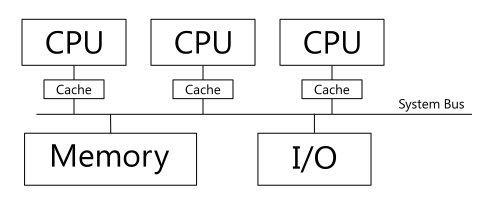
\includegraphics[resolution=96]{img/smp.png}
\caption{Схема многопроцессорной системы}
\end{figure}

В рамках курсовой работы будет производиться исследование функционирования
системы, состоящей из данного числа процессоров, постоянно принимающих задачи.
\begin{figure}[h]
\centering
\includegraphics[resolution=96]{img/sched_scheme.png}
\caption{Схема исследуемой системы}
\end{figure}

Задача курсовой работы состоит в исследовании данной системы при данных параметрах
процессоров и определения на основе параметров лучшей конфигурацию системы.

\subsection{Разработка концептуальной модели}
В рамках исследования будут использоваться следующие предположения и допущения:
\begin{enumerate}
\item Задачи поступают и уходят из очереди мгновенно.
\item Очередь имеет ограниченный размер, дисциплина обслуживания: roundrobin.
\item Задачи делятся на два класса приоритетов, основанных на абсолютных
приоритетах, во время выполнения процесса, его приоритет уменьшается с каждым
тактом.
\item Дисциплина прерывания -- прерванная задача возвращается в очередь.
\item Задачи имеют два состояния: выполнение на процессоре, готовность.
\end{enumerate}
\begin{figure}[h]
\centering
\includegraphics[resolution=96]{img/sched_model.png}
\caption{Модель исследуемой системы}
\end{figure}

На вход поступают задачи, которые тут же попадают в свободные очереди для
процессоров. Процессор выделяет определенный квант на процесс, по истечении
которого процесс либо завершается, либо направляется в очередь того, процесса,
который меньше всего нагружен.

\section{Имитационная модель}
\subsubsection{Результаты имитационного моделирования}
За параметр варьирования было решено взять время между поступлениями процессов,
а также размер кванта.
Были проведены замеры для интервалов между поступлениями процессов для 100 мс,
200 мс, 300 мс.
При изменении размера кванта интервал был задан 100 мс.

\subsubsection{Anylogic}
\begin{figure}[h]
\centering
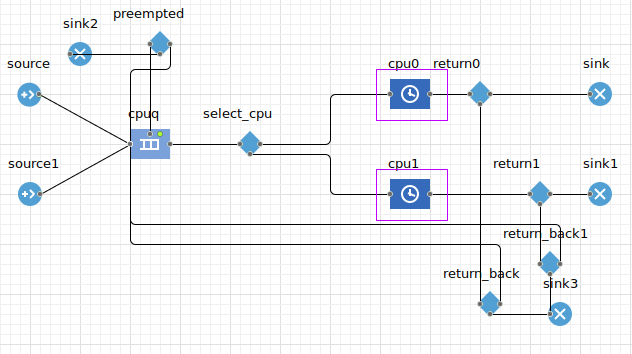
\includegraphics[resolution=96]{img/anylogic_model.png}
\caption{Модель Anylogic}
\end{figure}
\newpage
\subsubsection{GPSS}
\lstinputlisting{src/smo.gps.txt}
\subsubsection{Результаты Anylogic}

\begin{tabular}{|c|c|c|c|c|c|c|}
\hline
Время между поступлениями & Длина очереди & Загрузка прибора 1 & Загрузка прибора 2 \\ \hline
100 & 898,935 & 0,614 & 0,609 \\ \hline
 & 892,422 & 0,613 & 0,611 \\ \hline
 & 892,987 & 0,613 & 0,611 \\ \hline
 & 888,446 & 0,613 & 0,611 \\ \hline
200 & 4,871 & 0,497 & 0,51 \\ \hline
 & 4,875 & 0,492 & 0,497  \\ \hline
 & 4,755 & 0,492 & 0,495 \\ \hline
 & 4,896 & 0,498 & 0,501  \\ \hline
300 & 0,944 & 0,341 & 0,338  \\ \hline
 & 0,953 & 0,34 & 0,339 \\ \hline
 & 0,946 & 0,34 & 0,339 \\ \hline
 & 0,954 & 0,34 & 0,339  \\ \hline
\end{tabular}
\\

\begin{tabular}{|c|c|c|c|}
\hline
Размер кванта & Длина очереди & Загрузка прибора 1 & Загрузка прибора 2\\ \hline
100  & 879,948 & 0,612 & 0,611 \\ \hline
 & 892,422 & 0,611 & 0,61 \\ \hline
 & 892,987 & 0,611 & 0,61 \\ \hline
 & 888,446 & 0,611 & 0,61 \\ \hline
50 & 2,113 & 0,511 & 0,498 \\ \hline
 & 2,159 & 0,509 & 0,495 \\ \hline
 & 2,16 & 0,51 & 0,496 \\ \hline
 & 2,172 & 0,52 & 0,497 \\ \hline
10 & 0,029 & 0,108 & 0,109 \\ \hline
 & 0,028 & 0,107 & 0,108 \\ \hline
 & 0,03 & 0,108 & 0,109 \\ \hline
 & 0,029 & 0,108 & 0,109 \\ \hline

\end{tabular}

\subsubsection{Результаты GPSS}

\begin{tabular}{|c|c|c|c|}
\hline
Время между поступлениями & Длина очереди  & Загрузка прибора 1 & Загрузка прибора 2 \\ \hline
100 & 909,829 & 0,657 & 0,657 \\ \hline
 & 913,914 & 0,578 & 0,578 \\ \hline
 & 917,51 & 0,562 & 0,562 \\ \hline
 & 920,854 & 0,556 & 0,556 \\ \hline
200 & 17,305 & 0,514 & 0,514 \\ \hline
 & 16,244 & 0,513 & 0,513 \\ \hline
 & 17,135 & 0,514 & 0,514 \\ \hline
 & 16,984 & 0,513 & 0,513 \\ \hline
300 & 0,967 & 0,337 & 0,337 \\ \hline
 & 0,949 & 0,332 & 0,332 \\ \hline
 & 0,937 & 0,335 & 0,335 \\ \hline
 & 0,948 & 0,336 & 0,336 \\ \hline
\end{tabular}

\begin{tabular}{|c|c|c|c|}
\hline
Размер кванта & Длина очереди & Загрузка прибора 1 & Загрузка прибора 2 \\ \hline
100 & 909,829 & 0,657 & 0,657 \\ \hline
 & 913,914 & 0,596 & 0,588 \\ \hline
 & 917,51 & 0,597 & 0,597 \\ \hline
 & 920,854 & 0,554 & 0,554 \\ \hline
50 & 21,133 & 0,511 & 0,511 \\ \hline
 & 18,514 & 0,513 & 0,513 \\ \hline
 & 19,641 & 0,512 & 0,512 \\ \hline
 & 17,485 & 0,511 & 0,511 \\ \hline
10 & 0,014 & 0,099 & 0,099 \\ \hline
 & 0,012 & 0,101 & 0,101 \\ \hline
 & 0,012 & 0,102 & 0,102 \\ \hline
 & 0,013 & 0,1 & 0,1 \\ \hline
\end{tabular}
\subsection{Графические представления}
\begin{figure}
\centering
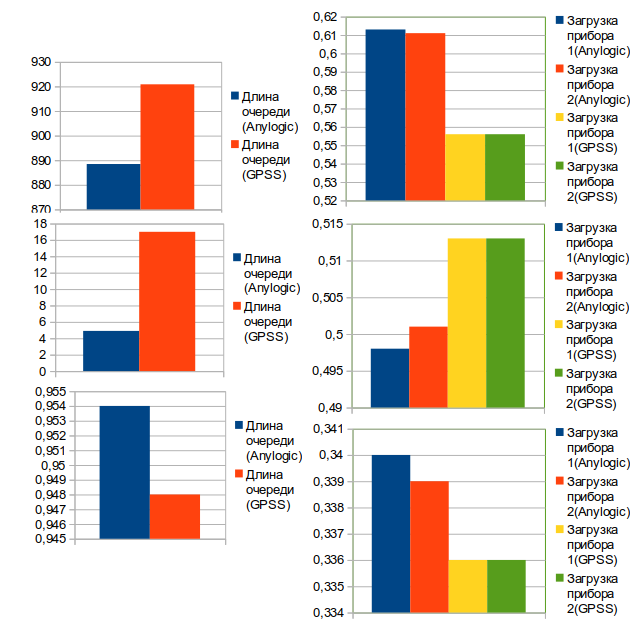
\includegraphics[resolution=96]{img/intensity.png}
\caption{Варьирование времени между процессами}
\end{figure}

\begin{figure}
\centering
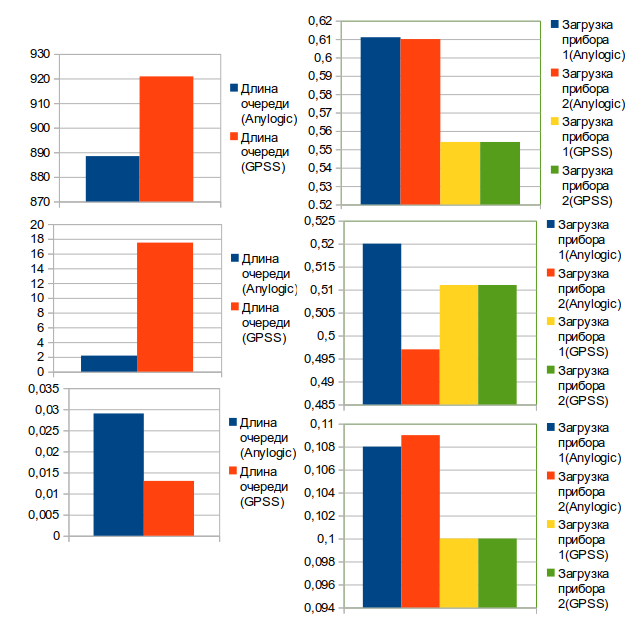
\includegraphics[resolution=96]{img/quantum.png}
\caption{Варьирование кванта} \end{figure}

\subsubsection{Доверительные интервалы}

\textbf{Anylogic}

\begin{adjustbox}{max width=\textwidth}
\begin{tabular}{|c|c|c|c|}
\hline
Время между поступлениями & Длина очереди & Загрузка прибора 1 & Загрузка прибора 2 \\ \hline
100 & 19,76092 & 0,00143 & 0,00287 \\ \hline
200 & 0,59952 & 0,00717 & 0,02023 \\ \hline
300 & 0,01174 & 0,00143 & 0,00143 \\ \hline
\end{tabular}
\end{adjustbox}
\newline
\vspace*{1 cm}
\newline

\textbf{Anylogic}

\begin{adjustbox}{max width=\textwidth}
\begin{tabular}{|c|c|c|c|}
\hline
Размер кванта & Длина очереди & Загрузка прибора 1 & Загрузка прибора 2 \\ \hline
100 & 18,30905 & 0,00143 & 0,00143 \\ \hline
50 & 0,06670 & 0,00248 & 0,00379 \\ \hline
10 & 0,00248 & 0,00143 & 0,00143 \\ \hline
\end{tabular}
\end{adjustbox}
\newline
\vspace*{1 cm}
\newline

\textbf{GPSS}

\begin{adjustbox}{max width=\textwidth}
\begin{tabular}{|c|c|c|c|}
\hline
Время между поступлениями & Длина очереди & Загрузка прибора 1 & Загрузка прибора 2 \\ \hline
100 & 9,54677 & 0,12635 & 0,12635 \\ \hline
200 & 1,41563 & 0,00143 & 0,00143 \\ \hline
300 & 0,03751 & 0,00625 & 0,00625 \\ \hline
\end{tabular}
\end{adjustbox}
\newline
\vspace*{1 cm}
\newline

\textbf{GPSS}

\begin{adjustbox}{max width=\textwidth}
\begin{tabular}{|c|c|c|c|}
\hline
Размер кванта & Длина очереди & Загрузка прибора 1 & Загрузка прибора 2 \\ \hline
100 & 9,54677 & 0,08678 & 0,09318 \\ \hline
50 & 3,26349 & 0,00248 & 0,00248 \\ \hline
10 & 0,00287 & 0,00379 & 0,00379 \\ \hline
\end{tabular}
\end{adjustbox}

\subsubsection{Выводы}
Результаты моделирования в разных программных продуктах показали хоть и различные,
но близкие, с учетом доверительного интервала, к друг другу результаты.
Вероятно, различия обусловлены разными реализациями генераторов случайных чисел
в каждой из программ.

По результатам моделирования видно, что при уменьшении времени между послуплениями
процессов, очередь начинает постоянно заполняться, так как помимо быстро приходящих
новых процессов, в очередь возвращаются процессы, отработавшие свой квант.

Для устранения этой проблемы можно как увеличивать время между поступлениями
процессов, так и изменять размер кванта, который выделяется на процесс. Однако,
как следует из результатов, при слишком маленьком кванте загрузка очень сильно
снижается, что приведет к слишком большим затратам на смену контекста в реальной модели.

Время между поступлениями процессов равное 200 мс можно назвать критическим,
т.к. при его уменьшении наблюдается постоянное увеличение размера очереди.

Подобрав наиболее удачные параметры кванта и времени поступления, можно сказать,
что данная система будет вести себя стабильно и при больших количествах процессов,
сохраняя высокую загрузку и малую длину очереди.


\newpage
\section{Аналитическая модель}
С помощью заданных допущений была составлена СМО с неоднородным потоком заявок,
ввиду того, что нагрузку нельзя свести к однородной из-за наличия приоритетов.

\subsection{Характеристики модели}

\begin{adjustbox}{max width=\textwidth}
\begin{tabular}{|c|c|c|c|c|c|c|c|c|c|c|c|c|c|}
\hline
\multicolumn{14}{|c|}{Характеристики обслуживания класса заявок в СМО} \\ \hline
& & \multicolumn{3}{|c|}{Ср. время ожидания} & \multicolumn{3}{|c|}{Ср. время пребывания} & \multicolumn{3}{|c|}{Ср. длина в очереди} & \multicolumn{3}{|c|}{Ср. число заявок в системе} \\ \hline
Класс & Загрузка & БП & ОП & АП & БП & ОП & АП & БП & ОП & АП & БП & ОП & АП \\ \hline
1 & 0,05 & 0,001 & 0,001 & 0,0003 & 0,301 & 0,301 & 0,3003 & 0,001 & 0,001 & 0,0003 & 0,101 & 0,101 & 0,1003 \\ \hline
2 & 0,05 & 0,001 & 0,0011 & 0,0018 & 0,301 & 0,3011 & 0,3018 & 0,001 & 0,0011 & 0,0018 & 0,101 & 0,1011 & 0,1018 \\ \hline
\end{tabular}
\end{adjustbox}
\\

\begin{adjustbox}{max width=\textwidth}
\begin{tabular}{|c|c|c|c|c|c|c|c|c|}
\hline
\multicolumn{9}{|c|}{Характеристики обслуживания объединенного потока заявок в СМО} \\ \hline
l & R & b & ДО & Ср. время ожидания & Ср. время пребывания & Ср. длина в очереди & Ср. число заявок в системе & Константа ВО \\ \hline
2 & 0,1 & 0,1 & БП & 0,001  & 0,301 & 0,002 & 0,202 & 0,00010 \\ \hline
 &  &  & ОП & 0,001 & 0,301 & 0,002 & 0,202 & 0,00011 \\ \hline
 &  &  & АП & 0,001 & 0,301 & 0,002 & 0,202 & 0,00011 \\ \hline

\end{tabular}
\end{adjustbox}

\subsubsection{Графики варьирования длительности обслуживания}

\begin{figure}[h]
\centering
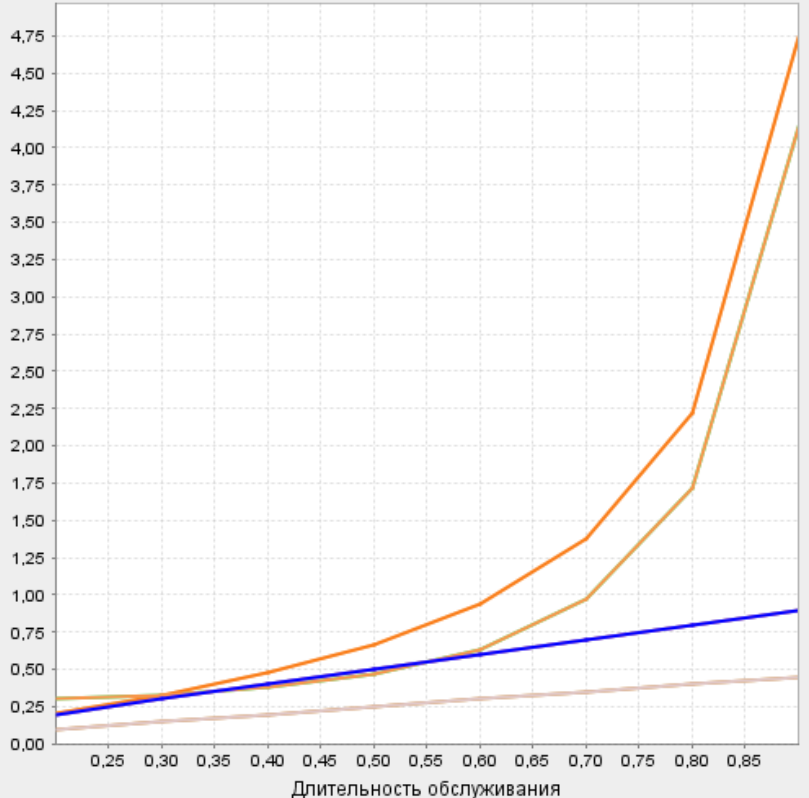
\includegraphics[resolution=200]{img/bp.png}
\caption{Без приоритетов}
\end{figure}

\begin{figure}[h]
\centering
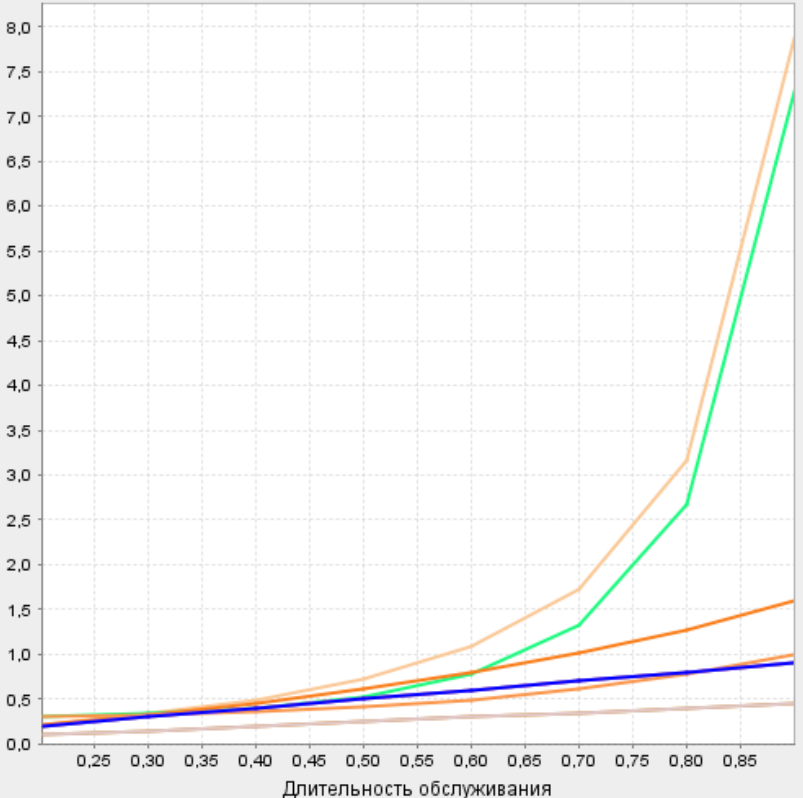
\includegraphics[resolution=200]{img/op.png}
\caption{Относительные приоритеты}
\end{figure}

\begin{figure}[h]
\centering
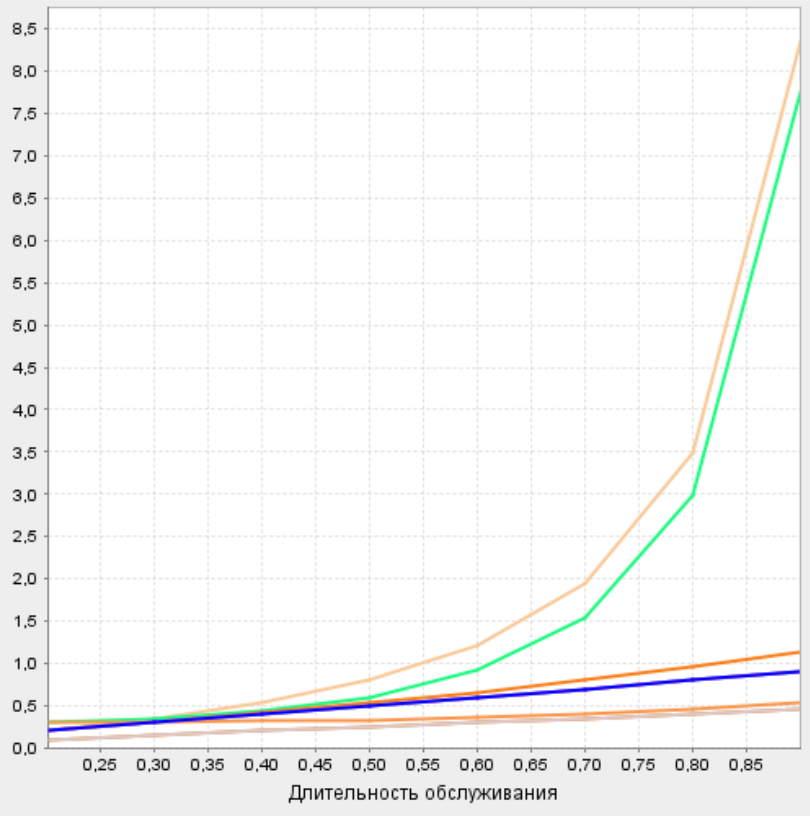
\includegraphics[resolution=200]{img/ap.png}
\caption{Абсолютные приоритеты}
\end{figure}

\subsubsection{Зависимости характеристик от приоритетов и от суммарной загрузки}
\begin{figure}[h]
\centering
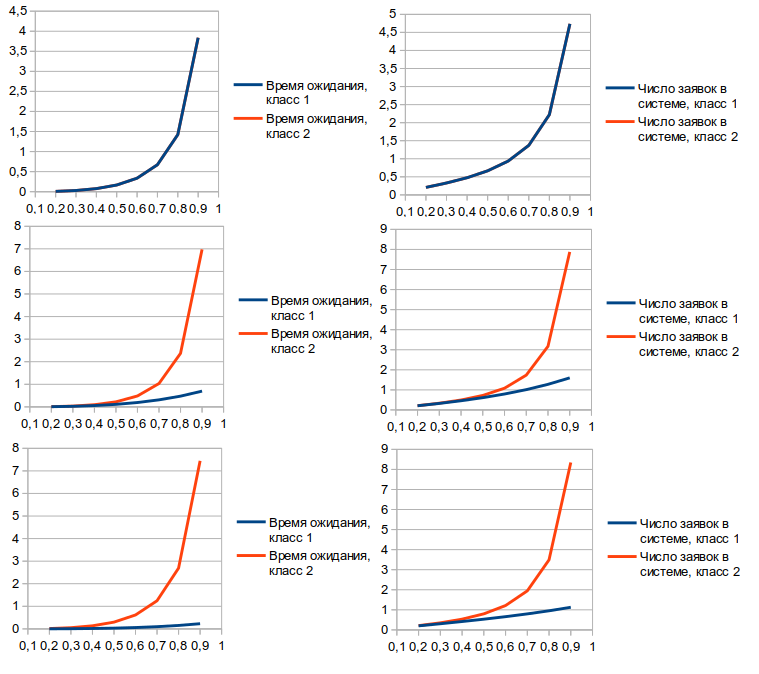
\includegraphics[resolution=128]{img/bp_op_ap_load.png}
\caption{БП, ОП, АП, от суммарной загрузки}
\end{figure}

\begin{figure}[h]
\centering
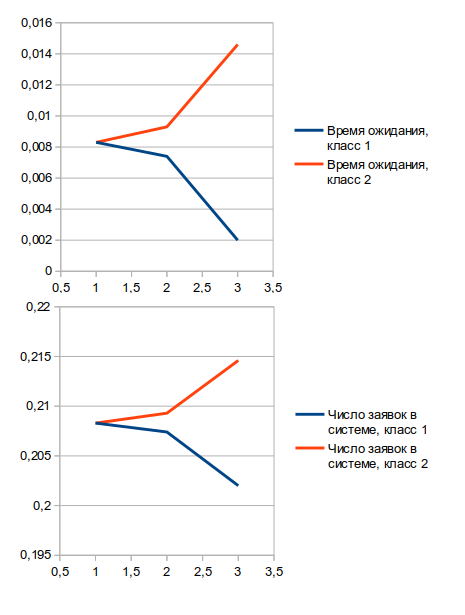
\includegraphics[resolution=128]{img/bp_op_ap_prio.png}
\caption{БП, ОП, АП, от приоритета}
\end{figure}

Исходя из графиков видно, что число заявок увеличивается для более приоритетного
класса 2, когда как для класса 1 оно уменьшается.
\end{document}
